\chapter{Badania}
\section{Źródła danych}
Podczas badań zostały przeprowadzone testy wydajności dla trzech operacji, które są reprezentowane przez końcowy interfejs użytkownika. Dokładny opis dostępu do danych znajduje się w sekcji \ref{sec:user_interfaces}. 
Na potrzeby badań operacje nazwijmy następująco:
\begin{itemize}
	\item {Word Count}
	\item {Filter}
	\item {Reject}
\end{itemize}
Testy wydajności zostały wykonane na danych zebranych poprzez Twitter Developer API opisanym w sekcji \ref{sec:twitter-api}. Z racji iż strumieniowanie dla platformy Spark zapisuje dane cyklicznie, powstał katalog w systemie HDFS zawierający paczki danych zapisanych co 360 sekund. Na potrzeby badań wszystkie dane pobrane ze zdalnego API zostały połączone w jeden plik o wielkości \textbf{4GB}, który posłużył za źródło danych podczas wykonywania testów wydajności. Twitter Developer API nie jest standardowym webowym interfejsem typu REST\footnote{Representational state transfer}. Nie występuje tutaj standardowy scenariusz zapytanie do serwera, odpowiedź serwera. W przypadku danych strumieniowych, klient wysyła zapytanie do aplikacji, aplikacja wysyła zapytanie do serwerów Twitter i czeka na odpowiedź serwera asynchronicznie. Klient wysyłając jedynie żądanie nie blokuje samego interfejsu aplikacji. W związku z tym może występować złudzenie iż klient nie posiada kontroli nad samym pobieraniem danych, gdyż raz wysłane żądanie nie może zostać przerwane. Aplikacja sama zarządza procesem pobierania/strumieniowania danych. Architektura o podobnej strategii jest proponowana również przez twórców samego Twitter Developer API i jest zaprezentowana na pod adresem: \url{https://dev.twitter.com/streaming/overview}.
\begin{figure}
	\centering
	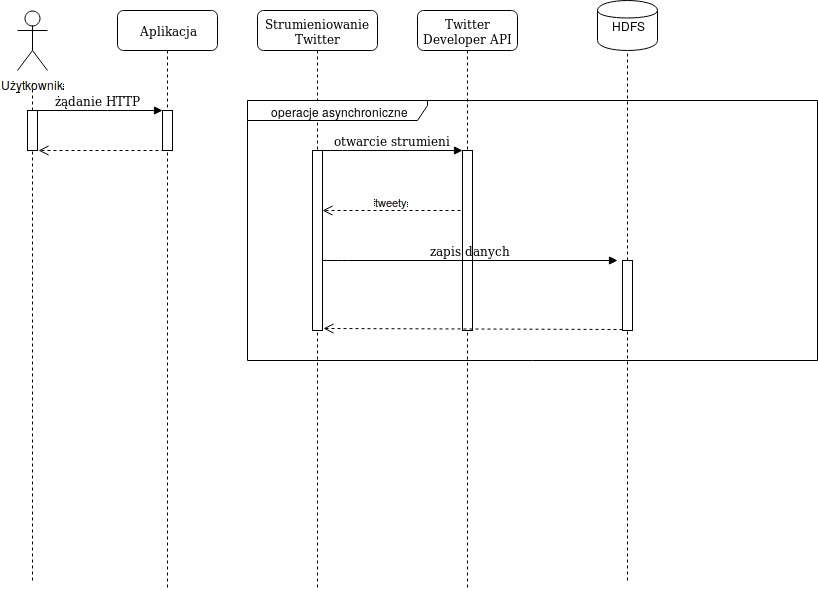
\includegraphics[scale=0.5]{twitter-api-connection.png}
	\caption{Architektura procesu pobierania danych z Twitter Developer API}
	\label{fig:@=twitter-api-connection}
\end{figure}
Proces strumieniowania danych z Twitter Developer API został przedstawiony na rysunku \ref{fig:@=twitter-api-connection}.

\section{Specyfikacja sprzętowa}
Badania zostały przeprowadzone na maszynie o specyfikacji:
\begin{itemize}
	\item Procesor: Intel Core i7-4702MQ (2.2GHz Quad-core + HT) 
	\item Pamięć RAM: 16GB
	\item Pamięć masowa: 1 TB 5400rpm\footnote{Revolutions per minute - obroty na minutę} SATA
	\item Karta graficzna: NVIDIA GeForce GT 750M (2G)  
\end{itemize}
Podczas badań specyfikacja karty graficznej nie ma wpływu na wyniki, gdyż dla badanych operacji wykorzystywane są trzy jednostki obliczeniowe: procesor, pamięć RAM, dysk twardy.
\newline Pomiary wydajności zostały dokonane przy pomocy programu \textbf{cURL}.\footnote{\url{https://curl.haxx.se/}} Testy obejmują siedem następujących czynników:
\begin{itemize}\label{items:time-descriptions}
	\item{Czas rozwiązywania adresu\footnote{time\_namelookup}}
	\item{Czas połączenia TCP\footnote{time\_connect}}
	\item{Czas wymiany informacji między połączeniami (handshake)\footnote{time\_appconnect}} 
	\item{Czas całkowity przed wymianą informacji\footnote{time\_pretransfer}}
	\item{Czas przekierowań\footnote{time\_redirect}}
	\item{Czas przed którym pierwszy bajt danych miał zostać wysłany\footnote{time\_starttransfer}}
	\item{Czas całkowity\footnote{time\_total}}
\end{itemize}
\todo{konfiguracja hadoop i spark - jaki tryb (lokalny), jaki tryb klastra}
\section{Wyniki}
Dla operacji \textit{Word Count} wyniki wydajności są przedstawione w tabeli \ref{tab:word-count-results}. 
\begin{table}[]
	\centering
	\caption{Wyniki wydajności dla zliczania ilości wystąpień poszczególnych fraz tekstowych (oddzielonych spacją) znalezionych w źródle danych oraz zapisu wyniku do pliku}
	\label{tab:word-count-results}
	\begin{tabular}{|l|l|l|}
		\hline
		Czas w sekundach    & Hadoop     & Spark      \\ \hline
		time\_namelookup    & 0.000020   & 0.000023   \\ \hline
		time\_connect       & 0.000097   & 0.000116   \\ \hline
		time\_appconnect    & 0.000000   & 0.000000   \\ \hline
		time\_pretransfer   & 0.000116   & 0.000134   \\ \hline
		time\_redirect      & 0.000000   & 0.000000   \\ \hline
		time\_starttransfer & 402.792577 & 111.232410 \\ \hline
		time\_total         & 402.792625 & 111.232446 \\ \hline
	\end{tabular}
\end{table}
Dla operacji \textit{Filter} wyniki wydajności są przedstawione w tabeli \ref{tab:filter-results}.
\begin{table}[]
	\centering
	\caption{Wyniki wydajności dla zliczania ilości linii zawierających frazę tekstową zdefiniowaną przez użytkownika}
	\label{tab:filter-results}
	\begin{tabular}{|l|l|l|}
		\hline
		Czas w sekundach    & Hadoop    & Spark     \\ \hline
		time\_namelookup    & 0.000022  & 0.000029  \\ \hline
		time\_connect       & 0.000090  & 0.000113  \\ \hline
		time\_appconnect    & 0.000000  & 0.000000  \\ \hline
		time\_pretransfer   & 0.000110  & 0.000140  \\ \hline
		time\_redirect      & 0.000000  & 0.000000  \\ \hline
		time\_starttransfer & 42.685888 & 16.489812 \\ \hline
		time\_total         & 42.685924 & 16.489860 \\ \hline
	\end{tabular}
\end{table}
Dla operacji \textit{Reject} wyniki wydajności są przedstawione w tabeli \ref{tab:reject-results}.
\begin{table}[]
	\centering
	\caption{Wyniki wydajności odrzucenia linii zawierających frazę tekstową zdefiniowaną przez użytkownika oraz zapisania wyniku do pliku}
	\label{tab:reject-results}
	\begin{tabular}{|l|l|l|}
		\hline
		Czas w sekundach    & Hadoop     & Spark     \\ \hline
		time\_namelookup    & 0.000025   & 0.000049  \\ \hline
		time\_connect       & 0.000098   & 0.000184  \\ \hline
		time\_appconnect    & 0.000000   & 0.000000  \\ \hline
		time\_pretransfer   & 0.000118   & 0.000237  \\ \hline
		time\_redirect      & 0.000000   & 0.000000  \\ \hline
		time\_starttransfer & 238.408629 & 45.186254 \\ \hline
		time\_total         & 238.408673 & 45.186296 \\ \hline
	\end{tabular}
\end{table}
\section{Interpretacja wyników}
Z punktu widzenia badanej wydajności wszystkie pomiary poza \textbf{time\_starttransfer} oraz \textbf{time\_total} nie są kluczowe gdyż pomijają czas pracy badanych platform. Czas całkowity jest interesujący z punktu widzenia użytkownika systemu, którego interesuje faktyczny czas uzyskania wyników. Podczas interpretacji wyników mylący może być opis przedstawiony w \ref{items:time-descriptions} \textit{Czas przed którym pierwszy bajt danych miał zostać wysłany}. Opis ten nie dotyczy danych, które są przetwarzane na badanych platformach lecz danych wysłanych przez odpowiedź na żądanie HTTP. Oznacza to, że dane odpowiedzi zostały wysłane po czasie gdy wszystkie obliczenia na platformie zostały już wykonane. W związku z tym \textbf{time\_starttransfer} może zostać uznany za czas pracy przetwarzania na danej platformie.
\newline W związku z wynikami przedstawionymi w tabelach \ref{tab:filter-results}, \ref{tab:reject-results}, \ref{tab:word-count-results} możemy zaobserwować zależność, że platforma Spark jest zdecydowanie szybsza (od dwóch i pół do pięciu razy) jeżeli chodzi o wykonywanie obliczeń i zapis wyników do pliku w systemie HDFS. Porównanie wydajności wszystkich operacji jest przedstawione na \ref{fig:results-comparison-bar}
\begin{figure}[!htb]
	\centering
	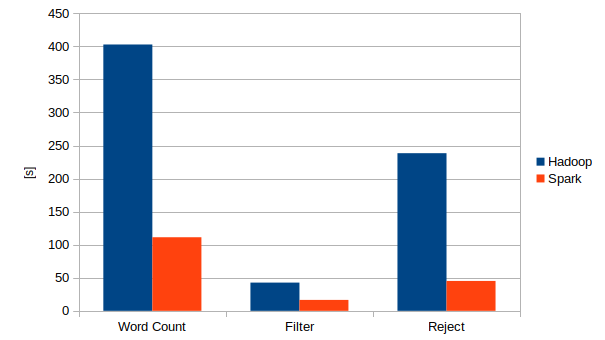
\includegraphics[scale=0.4]{results-comparison-bar.png}
	\caption{Wyniki wydajności operacji: Word Count, Filter i Reject}
	\label{fig:results-comparison-bar}
\end{figure}   
\todo{koszty rekrutacji, cyclomatic complexity?}